\documentclass{article}
\usepackage{amsmath}
\usepackage{empheq}
\usepackage{graphicx}
\begin{document}
\title{
\Huge\textbf{Discrete Assignment}\\
\Huge\textbf{EE1205} Signals and Systems\\
}
\large\author{Praful Kesavadas\\EE23BTECH11049}
\maketitle
\textbf{Question 11.9.1.2:}
Write the first five terms of the sequence whose $n^{th}$ terms  $x(n) = \frac{n}{n+1}$\\
\textbf{Solution:}
Given the terms of the sequence are $x(n) = \frac{n}{n+1}$ where $n = 0,1,2,3,4...$\\
In terms of $u(n)$, $x(n)$ is\\
\begin{align}
x(n) = u(n) -\frac{u(n)}{n+1}
\end{align}
\begin{align*}
    x(n) = 
    \begin{cases}
        0 & \text{if }n=0\\
        u(n) -\frac{u(n)}{n+1} & \text{if }n > 0\\
        \text{not defined } & \text{if }n <0
    \end{cases}
\end{align*}\\
Z-transform is defined as, 

$$ x(n) \xleftrightarrow Z  X(Z)$$

\begin{align}
X(Z) =  \sum_{i=-\infty}^\infty\ x(n).Z^{-n}\
\end{align}
Here, Z-transform
\begin{align}
X(Z) = \sum_{i=1}^\infty\ x(n).Z^{-n}
\end{align}
\begin{align}
= \sum_{i=1}^\infty \frac{n}{n+1} . Z^{-n}
\end{align}
On solving, 
\begin{align}
X(Z) = \frac{1}{1-Z^{-1}} + Z\log{(1-Z^{-1})}\
\end{align}
\begin{figure}[h]
    \centering
    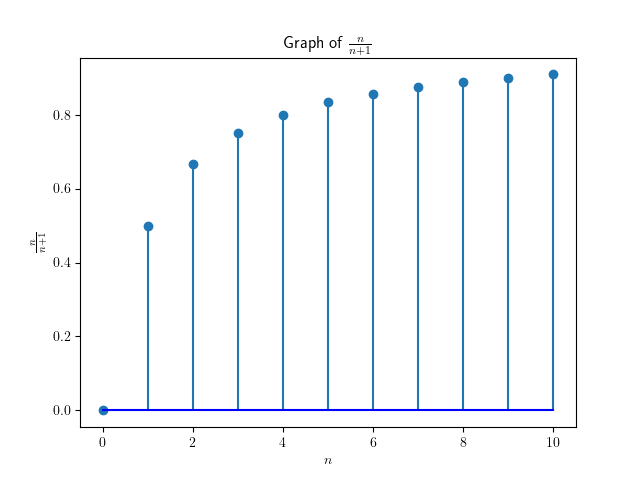
\includegraphics[width=0.7\linewidth]{graph.png}
    \caption{Sequence plot generated from Python script}
    \label{fig:sequence-plot}
\end{figure}
\end{document}
